\subsection{Experimentacion}

Para la experimentacion de backtracking se tomo de 6 a 40 nodos, y para cada familia de grafos se tomaron diferentes parametros para la misma cantidad de nodos. Los resultados fueron los siguientes:\\

\begin{figure}[ht]
\centering
	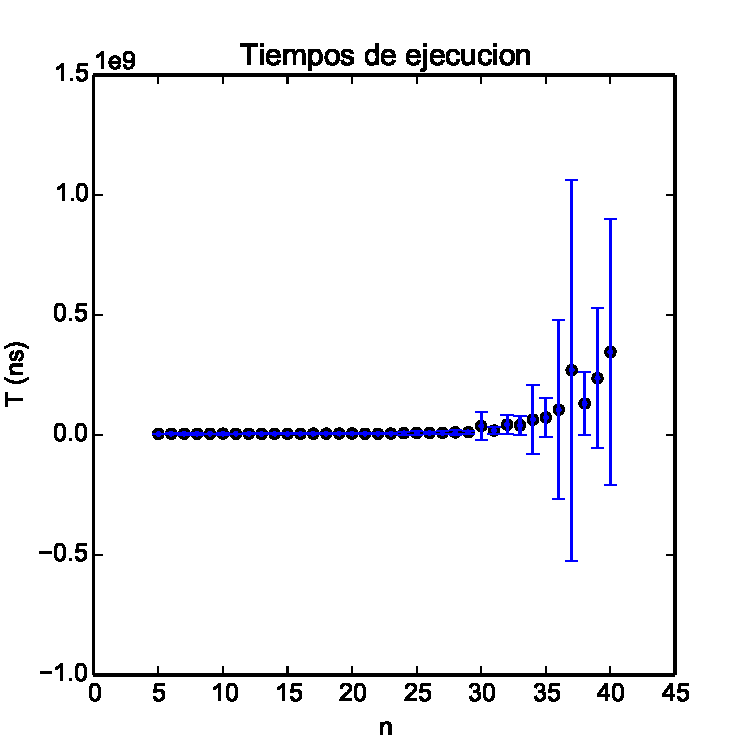
\includegraphics[scale=0.45]{images/graph_ej1/output_backtracking_1_n2}
	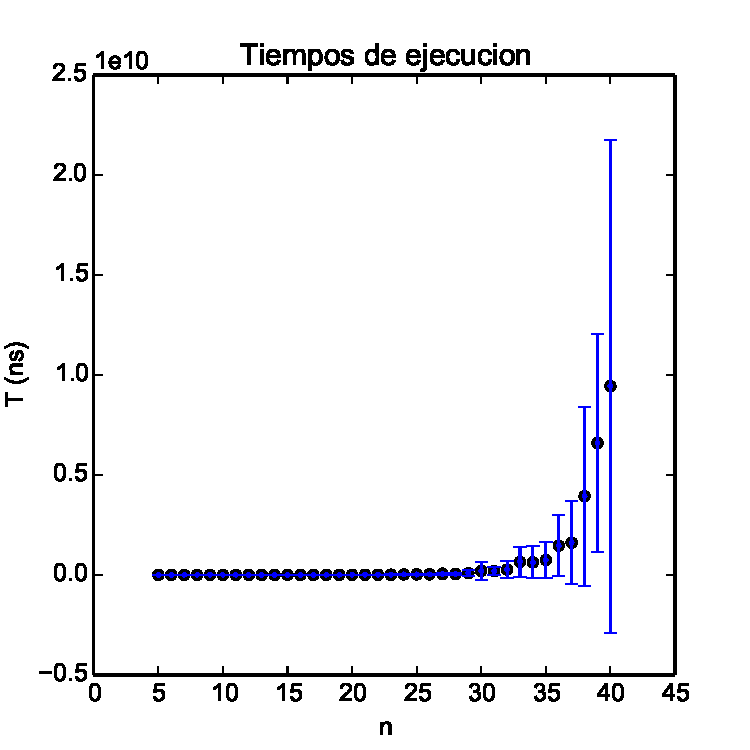
\includegraphics[scale=0.45]{images/graph_ej1/output_backtracking_1_n}
	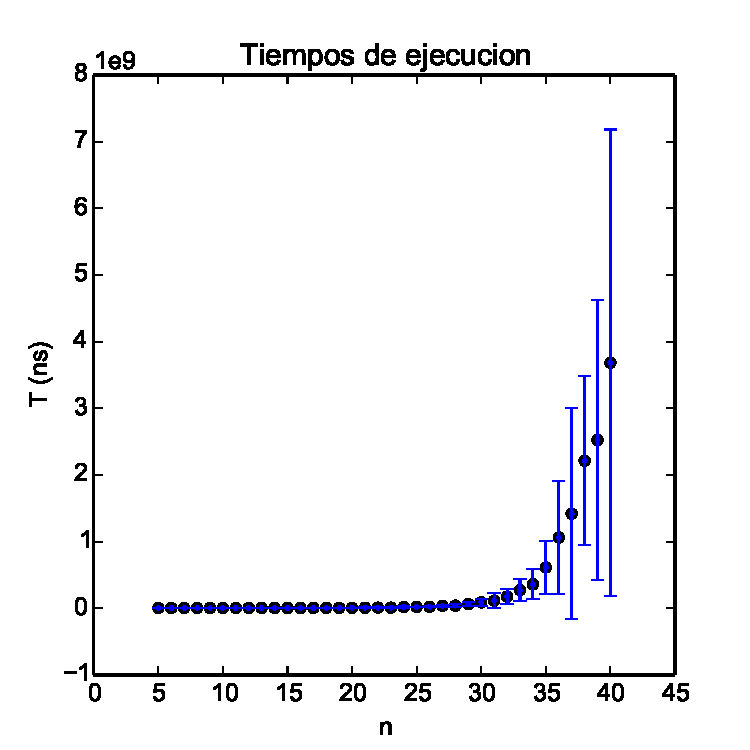
\includegraphics[scale=0.45]{images/graph_ej1/output_backtracking_1_2n}
\end{figure}